





\section{Elméleti alapok}

A dolgozatban használt terminológia, valamint a vizsgált rendszerek megértéséhez szükséges a kvantuminformatikában használt alapvető jelölések, valamint a kvantumos állapotok alapvető tulajdonságainak és a rajtuk végzett mérések, műveletek hatásainak ismerete. Ehhez nyújt egy gyors áttekintést a következő rész. Megjegyzendő, hogy jelen esetben a rendszereket csak diszkrét időben vizsgáljuk, mivel a későbbiekben vizsgált események leírásához ez elégséges, valamint hogy a bevezető megfelelő lineáris algebrai előismeretekre is épít.

\subsection{Posztulátumok:} 
A posztulátumokat a \cite{kvantkonyv1} irodalom alapján mutatom be.\\

\underline{1. posztulátum - állapotteres leírás:} Egy zárt fizikai rendszer éppen aktuális állapota leírható egy \textbf{V} Hilbert-térbeli egységhosszú, komplex együtthatós állapotvektorral. Hilbert-tér például egy komplex lineáris vektortér, amire értelmezve van a belső szorzat(skalárszorzat). 
Vegyünk példának egy két dimenziós Hilbert-teret, ami egy egyszerű zárt fizikai rendszert jelképez. A rendszer állapotát le lehet írni egy \textbf{v} két dimenziós vektorral, ahol:\\
\begin{center}
$ v= \begin{bmatrix} a\\b \end{bmatrix} = a\textbf{0}+ b\textbf{1} $ ,ahol 
$\textbf{0}=\begin{bmatrix} 1\\0 \end{bmatrix} , \textbf{1}=\begin{bmatrix} 0\\1 \end{bmatrix} ,   a,b \in C$
\end{center}
Itt \textbf{0} és \textbf{1} az orthonormális(ortgonális és egységhosszú) bázisvektorok. Mivel az állapotvektor egységhosszú, ezért ki kell még kötni, hogy 
$\abs{a}^2+\abs{b}^2 =1$ . Az együtthatókra szokás még valószínűségi amplitúdóként is hivatkozni (a Schrödinger hullámfüggvényben amplitúdóként jelennek meg).

\underline{2. posztulátum - rendszer időbeli fejlődése} Zárt fizikai rendszer időbeli fejlődése leírható csak a változás kezdő- és végpontjától függő unitér transzformációval. Az előbbi jelölésrendszer segítségével leírva: 
\begin{center}
$v'(t_2) = U(t_1,t_2)v(t_2), v' \in V$
\end{center}
$ U $ unitér operátor lineáris algebrai reprezentációja egy \textbf{U} kvadratikus mátrix, melynek $U_{ij}$ elemei a bemeneti \textbf{j} orthonormális bázisvektor \textbf{i} vektorral való kapcsolatát jelképező valószínűségi amplitúdókat jelölik.\\

\underline{3. posztulátum - mérés:} Méréseket leírhatunk $M_m$  mérési operátorokkal, ahol $m$ a lehetséges mérési eredményeket jelöli. $m$ mérésének a valószínűsége, ha a rendszer \textbf{v} állapotban van:
\begin{center}
$P(m|\textbf{v})= {\textbf{v}}^\dagger M_m^\dagger M_m \textbf{v} $
\end{center}
A rendszer állapota mérés után:
\begin{center}
$ {\textbf{v}}' = \frac{M_m \textbf{v}}{\sqrt{{\textbf{v}}^\dagger M_m^\dagger M_m \textbf{v}}}  $
\end{center}
Mivel a kimenetek összesített valószínűsége 1-el egyenlő(a lehetséges kimenetek lefedik a teljes eseményteret):
\begin{center}
$ \sum_m P(m|\textbf{v}) = \sum_m {\textbf{v}}^\dagger M_m^\dagger M_m \textbf{v} \equiv 1$
\end{center}
ami alapján:
\begin{center}
$\sum_m M_m^\dagger M_m \equiv I $
\end{center}
A mérések nem visszafordíthatóak és befolyásolják a mért rendszer állapotát a fentebb már leírt módon. Ugyanakkor velük teremthetjük meg a kapcsolatot a klasszikus és a kvantum világ között, mivel ők azok az eszközök,  amikkel megfigyelhetjük mégiscsak mi történik a kvantum világban.
\\
\underline{4. posztulátum - összetett rendszerek:}
Egy $ W $ összetett fizikai rendszer állapota leírható az őt összetevő rendszerek tenzorszorzataként:
$ W=V \otimes Y $ .Továbbá ha $\textbf{v} \in V  $  és  $ \textbf{y} \in Y $ akkor a belőlük alkotott állapot: $ \textbf{w}=\textbf{v}\otimes \textbf{y} $ .
A kvantummechanikában a legkisebb információt hordozó elem a bit, amit kvantumbitnek, vagy röviden qubitnek  szokás hívni. Egy qubit szokványos leírása:
\begin{center}
$ \ket{\psi}=a\ket{0}+b\ket{1}=a \begin{bmatrix}1\\0\end{bmatrix}+ b \begin{bmatrix}0\\1\end{bmatrix} = \begin{bmatrix} a\\b \end{bmatrix} $
\end{center}
A klasszikus számítástechnikához hasonlóan \textit{n} qubit felhasználásával építhetünk \textit{n} bites kvantumregisztereket. Vizsgáljunk például egy két qubitből alkotott kvantumregisztert. Ekkor a teljes két qubites rendszer állapota:
\begin{center}
$ \ket{\psi} \equiv \ket{\psi_1}\ket{\psi_2} \equiv \ket{\psi_1,\psi_2} \equiv \ket{\psi_1\psi_2} $
\end{center}
Ami például hogyha:
\begin{center}
$ \ket{\psi_1} = \frac{\ket{0}+\ket{1}}{\sqrt{2}}, \ket{\psi_2}=\frac{\ket{0}+\ket{1}}{\sqrt{2}}, $
\end{center}
akkor:
\begin{center}
$ \ket{\psi}= \frac{\ket{0} \otimes \ket{0} +\ket{0}\otimes\ket{1}+\ket{1}\otimes\ket{0}+\ket{1}\otimes\ket{1}  }{2} = \frac{\ket{00}+\ket{01}+\ket{10}+\ket{11}}{2} $
\end{center}
Látszik, hogy az előbbi rendszer a 00,01,10,11 állapotok (amelyek mellesleg ortogonálisak egymásra,itt az állapottér bázisának tekinthetőek) súlyozott (most itt mindegyik 1/2 -el de ez lehet bármilyen más komplex szám is, sőt akár 0 is.) összege, ezeket mind tartalmazza és jól látszik, hogy felbontható $\ket{\psi_1}$  és  $\ket{\psi_2}$  tenzorszorzatára. Az ilyen állapotokat hívjuk szorzat állapotoknak.\\
Most vizsgáljuk a következő állapotot:
\begin{center}
$ \ket{\psi} = a\ket{00}+b\ket{11} $
\end{center}
Ezt nem tudjuk felbontani két qubit tenzorszorzatára. Az ilyen állapotokat hívjuk összefonódott állapotnak. Vegyük észre ennek az állapotnak egy érdekes tulajdonságát! Ha megmérjük az egyik bitjét, akkor valamilyen valószínűséggel 0-át vagy 1-et kapunk. Viszont ha ezután megmérjük a másik bitet is, ha az első mérésünk eredménye 0 volt, akkor itt már csak 0-át mérhetünk és ehhez hasonlóan 1-es eredmény esetén pedig csak 1-et. Továbbá kísérletileg bizonyított, hogy ez a jelenség akkor is fenn marad, ha a rendszer két qubitjét helyileg egymástól eltávolítjuk.
Néhány nevezetes összefonódott állapot, amelyeket Bell-állapotoknak szokás nevezni:
\begin{center}
$ \ket{\Phi^-}= \frac{1}{\sqrt{2}}(\ket{0_A0_B}-\ket{1_A1_B}) $ \\
$ \ket{\Phi^+}= \frac{1}{\sqrt{2}}(\ket{0_A0_B}+\ket{1_A1_B}) $ \\
$ \ket{\Psi^-}= \frac{1}{\sqrt{2}}(\ket{0_A1_B}-\ket{1_A0_B}) $ \\
$ \ket{\Psi^+}= \frac{1}{\sqrt{2}}(\ket{0_A1_B}+\ket{1_A0_B}) $ \\

\end{center}

Figyeljük meg, hogy ezek az állapotok egymásra merőlegesek, az állapotérnek bázisaiként szolgálhatnak. Ennek segítségével definiálhatjuk az ún. Bell-mérést ami egy 2 qubites rendszer projektív mérése ezekben a bázisokban. Megjegyzendő még, hogy a mérés után a mérési posztulátumnak megfelelően a két qubit a négy Bell-állapot egyikébe kerül.\\
Megjegyzés: A kapcsolódó irodalmak olvasásához szükséges lehet még a sűrűségmátrixos leírás ismerete (lsd. \hyperref[suru]{F. 1.}), viszont a dolgozat olvasáshoz nem, ezért ennek ismertetésétől eltekintettem.\\

\section{Összefonódás megosztás}
%(entanglement swapping)
\subsection{A jelenség bemutatása}
Az összefonódott állapotok érdekes tulajdonságait természetesen igyekszünk kihasználni a kvantuminformatikában is, nem véletlen tehát, hogy magára az összefonódásra is mint egy fontos erőforrásként tekinthetünk. Elég csak olyan, protokollokra gondolni, mint a szupersűrűségű kódolás, vagy a kvantumteleportáció, melyek mind összefonódott állapotokat “használnak el” a működésük során. Nem csoda tehát, hogy egy adott helyen(vagy helyek között) való összefonódás létrehozásának képessége különös jelentőséggel bír. Ezzel kapcsolatban létezik szerencsére egy számunkra igen hasznos és viszonylag sokszor hasznosított jelenség, az összefonódás megosztás (entanglement swapping), mellyel egy összefonódott párok közötti érdekes interakciót írunk le. A már 1993-ban felvetett koncepció szerint \cite{zukowski1993event} 2 összefonódott pár interakcióját vizsgáljuk egymással a következő módon.A példában tekintsünk kvantum információ hordozóira fotonokként, de természetesen minden fotonhoz hasonló kvantum információ hordozására alkalmas módszerre is az alábbiak szerinti a jelenség. Az összefonódott párjaink közül az egyik kezdetben legyen Alíznál, a másik pedig Bobnál. Legyen a rendszerünk kezdő állapota:
\begin{center}
$ \ket{\Psi_{kezd}^-}= \ket{\Psi^-}_{AB} \otimes \ket{\Psi^-}_{CD} $
\end{center}
ahol $ \Psi^- $ a már fentebb említett Bell állapot, AB fotonpár van Alíznál és CB fotonpár pedig Bobnál.A teljes állapot felírható:
\begin{center}
$ \ket{\Psi_{kezd}^-} = \frac{1}{2} \Big( \ket{\Psi^+}_{AD}\ket{\Psi^+}_{BC}-\ket{\Psi^-}_{AD}\ket{\Psi^-}_{BC} - \ket{\Phi^+}_{AD}\ket{\Phi^+}_{BC}+\ket{\Phi^-}_{AD}\ket{\Phi^-}_{BC} \Big) $
\end{center}
(Részletesebb magyarázatért lsd. \hyperref[osszfonmeg]{F. 2.})\\
Alíz elküldi A fotont Bobnak, Bob pedig C fotont Alíznak, tehát Alíznál lesz B és C, míg Bobnál A és D. Ha Alíz Bell mérést hajt végre BC fotonpárján és $ \ket{\Psi^-}_{BC} $  állapotban találja, akkor ha Bob is megméri a saját párját $ \ket{\Psi^-}_{AD} $ állapotot fog találni. Ha Alíz a mérése során a maradék három állapot közül találja valamelyiket, akkor Bob ennek megfelelő állapotokat fog találni az ő fotonpárja mérésénél is. Látszik, hogy a Bobnál előfordulható állapotok mind tiszta összefonódott állapotok, emiatt ha Alíz Bell mérést végez, tudhatjuk, hogy a Bobnál lévő fotonpár össze van fonódva Alíz mérési eredményének pontos ismerete nélkül. Érdemes megfigyelni, hogy a Bobnál lévő fotonok semmilyen közös múlttal nem rendelkeznek, mégis szert tettek egy közös tulajdonságra, összefonódott állapotba kerültek.
\begin{figure}[H]
\centering
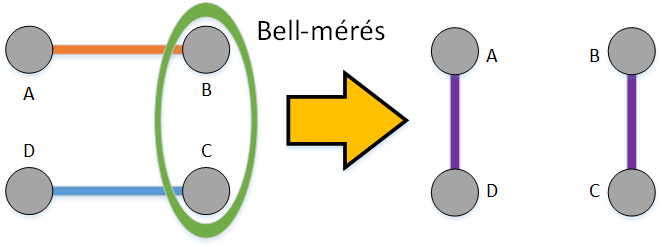
\includegraphics[width=110mm, keepaspectratio]{entanglementswapping2}
\caption[Összefonódás megosztás]{Összefonódás során a párok változása. Bal oldalt a Bell-mérés előtti állapot, jobb oldalt a mérés utáni. A mérést B és C biteken végezzük el.}
\end{figure}
A folyamatot lehet úgy is tekinteni, mintha a kvantumteleportációs protokoll \cite{bennett1993teleporting} segítségével egy már kezdetben is összefonódott állapot egyik kvantumbitjét teleportáltuk volna, csak ebben az esetben nem a kiválasztott kvantumbit pontos átvitele a fontos, hanem csak az összefonódás, mint a két kvantumbites rendszerre jellemző állapot, továbbítása az. Alíz mérési eredményének pontos ismerete és a feltételes visszaállító transzformációk, továbbá az ehhez szükséges 2 klasszikus bitnyi információ itt nem is része  a folyamatnak, mivel fentebb már megmutattuk, hogy az összefonódás léte (ami most minket érdekel) ezek nélkül is belátható.
\\
\begin{figure}[H]
\centering
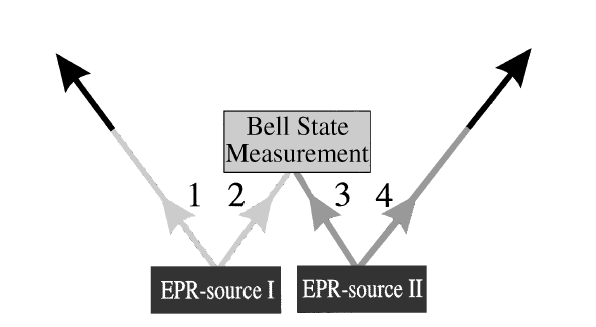
\includegraphics[width=100mm, keepaspectratio]{osszfonmeg1}
\caption[Összefonódás megosztás elvi rajza]{Összefonódás megosztás elvi rajza: Két összefonódott pár forrás (EPR source I és II) összefonódott fotonpárokat bocsájt ki(1-2 és 3-4). Mindegyik párból 1-1 fotonnal (2 és 3) végrehajtunk egy közös Bell mérést, aminek hatására a maradék két foton(1 és 4) is összefonódott állapotba kerül.}
\end{figure}
Megjegyzendő még érdekességként, hogy Peres elméletének megfelelően \cite{peres2000delayed} az összefonódás megosztás akkor is végbemehet, ha a (jelen esetben Alíznál) Bell mérést csak azután hajtjuk végre, hogy Bobnál már megmértük a másik két(jelen példánál A és D) állapotokat. Ezt igazolja például egy 2012-es kísérlet is \cite{ma2012experimental}.
\\
\begin{figure}[H]
\centering
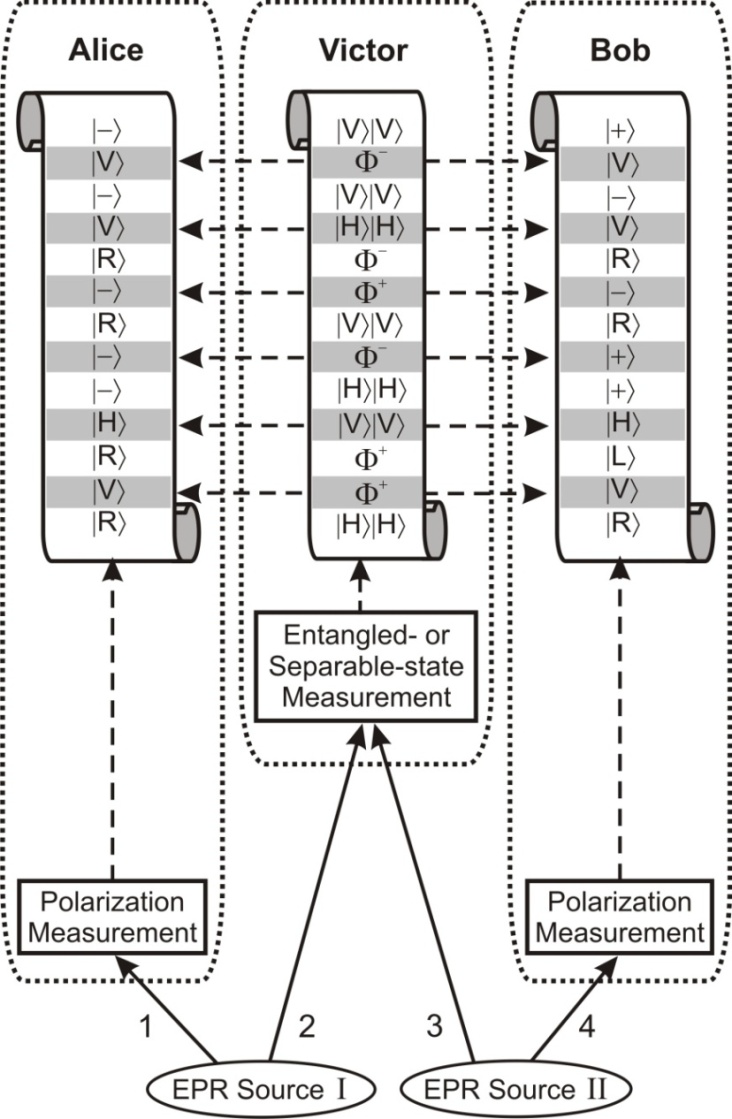
\includegraphics[width=100mm,keepaspectratio]{delayedchoice}
\caption[Késleltetett összefonódás megosztás kísérlet]{Elvi kísérleti összeállítás delayed choice(késleltetett döntéses) összefonódás megosztás vizsgálatára. Az előzőekhez hasonlóan itt is két összefonódott pár forrás szolgáltatja a fotonpárokat, viszont a korábbiakkal ellentétben itt először az 1-es és 4-es foton állapotait nézzük meg, utána véletlenszerűen döntünk, hogy Bell mérést, vagy valamilyen szétválasztható állapot szerinti mérést végzünk el. Ezek után Alíz és Bob rendezni és vizsgálni tudja a már meglévő mérési adatait Victor döntése ismeretében. Azt kapjuk, hogy Alíz és Bob fotonjai vagy összefonódott vagy szétválasztható állapotokként viselkednek, Victor mérési eredményeinek megfelelően.}
\end{figure}

\subsection{Összefonódás megosztások összefűzése}

Tekintve, hogy milyen fontos szerepe van az összefonódásnak a kvantumkommunikáció területén, az összefonódás megosztás is egy fontos eljárása, építőeleme számos kvantumkommunikációs protokollnak. Ezek közül talán az egyik legfontosabb ilyen felhasználási terület
a kvantum ismétlők (quantum repeaters). A kvantumkommunikációs csatornák a valóságban nem tekinthetőek tökéletesnek, hasonlóan a klasszikus összeköttetésekhez, itt is számolni kell például csillapítással (hosszabb távon komoly probléma például a fotonok elnyelődése, detektálásuk nehézsége), a környezet hatásaival, mint például dekoherencia, zaj. Ebből adódóan nem élhetünk azzal a feltételezéssel, hogy hosszabb kapcsolatoknál az elküldött információnk a fogadó oldalra eredeti formájában jut el. A kvantum csatorna átvitelére jellemző exponenciális csökkenés pedig gyakorlatilag ellehetetleníti a hosszabb távokon át történő információátvitelt. Erre lehetne az egyik megoldás, a klasszikus kommunikációhoz hasonlóan, ha megfelelően nem túl nagy távolságonként ismételnénk, eredeti állapotában mindig újra küldenénk tisztábban a küldendő bitet. A klasszikus kommunikációban ez könnyedén megoldható, azonban a kvantumos másolási tétel (No Cloning Theory) miatt nem lehet azt a megoldást teljes egészében lemásolni. Vegyük észre viszont, hogy a kvantum teleportációs protokoll segítségével tetszőleges állapotot tudunk elvinni egyik helyről a másikra, feltéve hogy a cél és a forrás rendelkezik egy összefonódott párral amin már előzőleg megosztoztak. A problémát ily módon vissza tudjuk vezetni összefonódott párok szétosztására (mert klasszikus információt már tudunk nagy távolságokra is szállítani). Összefonódott párokat különben sem csak a teleportációs protokoll használ működése során, két hely közötti összefonódásra tekinthetünk egy általában is értékes erőforrásként. Itt lehet segítségünkre az összefonódás megosztás jelentősége.  \\
 
Természetesen ha összefonódott párokat akarunk szétosztani ugyanúgy fennállnak az előzőleg említett problémák a csatornával, viszont tekintsük a következő esetet \cite{goebel2008multistage}: Ha az összefonódott párok közül az egyiket előzőleg összefonódás megosztásával hozzuk létre, könnyen elképzelhető, egy szabadon bővíthető séma, ahol a nagy átviteli távolságot, többszöri összefonódás megosztásával több kisebb szakaszra lehet bontani.
Vizsgáljuk meg azt az esetet amikor ezt a hosszabb távot két részre osztjuk fel. Ilyenkor kétszer kell összefonódást megosztani, három összefonódás forrásunk van, és két Bell-mérést hajtunk végre a párjainkon. Ha a párjaink kezdetben 1-2 3-4 és 5-6, akkor Bell-méréseket hajtunk végre 2-3-on és 4-5-ön. Ennek eredményeként 1 és 6 kerül összefonódott állapotba.
\\

\begin{figure}[H]
\centering
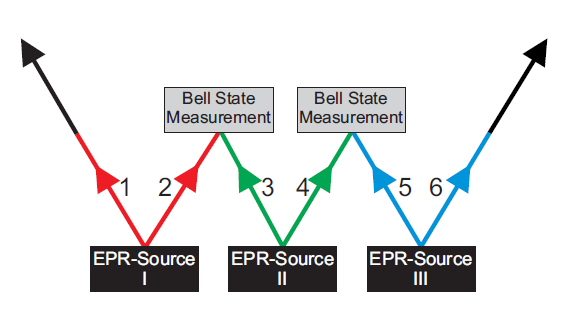
\includegraphics[width=120mm,keepaspectratio]{swapconcat}
\caption[Összefonódás megosztások összefűzése]{Többlépcsős összefonódás megosztás elvi felépítése:\\
A források által (EPR-Source I-II-III) kiadott kezdeti összefonódott párok: 1-2, 3-4, 5-6. 2 és 3-on majd 4 és 5-ön elvégezzük a Bell mérést. A két Bell mérés hatására végül 1 és 6 kerül összefonódott állapotba.}
\end{figure}

Felírva a rendszer állapotát:
\begin{center}
$ \ket{\Psi}_{123456}= \ket{\Psi^-}_{12} \otimes \ket{\Psi^-}_{34} \otimes \ket{\Psi^-}_{56} $
\end{center}
Ez átírható a következő alakra:
\begin{center}
$ \ket{\Psi}_{123456} = \frac{1}{2} \Big[ \ket{\Psi^+}_{14}\ket{\Psi^+}_{23}-\ket{\Psi^-}_{14}\ket{\Psi^-}_{23}-\ket{\Phi^+}_{14}\ket{\Phi^+}_{23} + \ket{\Phi^-}_{14}\ket{\Phi^-}_{23} \Big] \otimes \ket{\Psi^-}_{56} $
\end{center}
A korábbi két fotonpáros esethez hasonlóan itt is megfigyelhető, hogy az 1-es és 4-es fotonok az első Bell-mérés után összefonódott állapotba kerülnek a mérés eredményétől függetlenül. Az eredmény csak arról szolgáltat információt, hogy melyik összefonódott állapotban vannak, mivel az most is egyezik 2-3 közös mért állapotával.
Ha feltesszük, hogy 2-3-as fotonpárnál $ \ket{\Phi^-} $   állapotot mértünk, a fennmaradó 4 fotonos rendszer a továbbiakban a következő formában írható fel:
\begin{center}
$ \ket{\Psi}_{1456} = \frac{1}{2}\Big[ \ket{\Psi^+}_{16}\ket{\Phi^-}_{45}+\ket{\Psi^-}_{16}\ket{\Phi^+}_{45} - \ket{\Phi^+}_{16}\ket{\Psi^-}_{45} - \ket{\Phi^-}_{16}\ket{\Psi^+}_{45} \Big] $
\end{center}
Hasonlóan az előzőekhez, elvégezzük a Bell mérést 4-5-ön, aminek hatására 1 és 6 összefonódott állapotba kerül. A mérési eredménynek megfelelően például, ha a Bell mérésnél $\ket{\Phi^-} $ állapotot mérünk, akkor 1-6-nak az állapota: $ \ket{\Psi^+} . $ \\
A folyamat a fentiekből kiindulva általánosítható több tetszőleges számú összefonódott párra, tetszőleges számú Bell-méréssel, amivel az áthidalni kívánt távolság is tetszőleges számú szakaszra bontható fel.\\
A itt ábrázolt módszer is még idealizált csatornákkal dolgozik, magában nem oldja az előzőleg említett problémákat, mégis egy fontos építőeleme a későbbi ismétlő létrehozására irányuló modelleknek.
%%%
\subsection{A kvantum ismétlő}
%%%
A kvantum ismétlő megvalósítására törekvő modellek túlnyomó része három fő építőelemből áll, és jellemzően e három építőelem más és más megvalósításában tér el egymástól. Egy jellemző általános megvalósítás az alábbi:
A nagy távolságon jelentkező romlás elkerülése végett, ezt a távolságot felosztjuk több kisebbre, amik között a fentebb részletezett módon összefonódás megosztással teremtünk kapcsolatot. A felosztott kis távolságok között állomásokat alakítunk ki (ismétlőket). Itt végezzük el az összefonódás megosztáshoz szükséges Bell-méréseket. Ezen felül minden szakaszhoz (minden összefonódás megosztási lépcsőhöz) létre kell hoznunk plusz összefonódott párokat amiket a folyamat során elhasználunk.\\
 Ehhez szükségünk van egy összefonódott pár forrásra, ami manapság már igen sokféle lehet. %források jöhetnek még ide
Ez az egyik fő hasonlóság és egyben különbség is a legtöbb megvalósításban. A források maguk is sokféle karakterisztikával rendelkezhetnek. Adhat ki egy forrás kis sebességgel, nagy hibaszázalékkal közel teljesen tiszta állapotokat, vagy akár nagyobb sebességgel kisebb hibaszázalékkal több kevésbé tiszta állapotot is egyszerre.\\
 A csatorna nem ideális átvitelével is foglalkozni kell, látható, hogy az továbbra is exponenciálisan fog romlani a csomópontok közötti hossz növelésével. Ennek kiküszöbölésére használhatunk valamilyen összefonódás tisztító eljárást.\\
 Ezek jellemzően több nem teljesen tiszta összefonódott állapotból állítanak elő kevesebb, tisztább, jobban összefonódott állapotokat. Tipikusan van egy tisztasági határérték a felhasznált “koszos” összefonódott állapotokra ami fölött alkalmazhatóak, emiatt akár ezek paraméterei is támaszthatnak határokat a csatornaszakaszok hossza felé. Segítségükkel az átviteli sebesség kárára ugyan, de az átviteli folyamatok közé megfelelően beiktatva, kompenzálhatóak a csatornából származó veszteségek. Ennek szemléltetésére vizsgáljunk egy egyszerűbb ilyen eljárást.\\
\underline{Példa egy tisztító protokollra:}\\
Egy lehetséges ilyen tisztító protokoll például a Bennett által javasolt protokoll\cite{bennett1996purification} amelyben helyben végzett transzformációk segítségével több nem teljesen “tiszta” összefonódott párból kevesebb jobban összefonódott állapot hozható létre. (Megemlítendő, hogy eredetileg elektronspinekre írták le, de természetesen megvalósítható más hordozók esetén is.) Legyen $M$ egy “kevert”(nem tiszta) állapot amiből tisztább, jobban összefonódott állapotokat szeretnénk létrehozni. (Ilyen lehet például egy zajos csatornán megosztott $ \ket{\Psi^-} $  pár.) Ilyenkor $M$ tisztaságát az eredeti teljesen összefonódott állapothoz képest 
$ F= \bra{\Psi^-}M\ket{\Psi^-} $ 
segítségével fejezhetjük ki. Ezt akár értelmezhetjük azzal is ebben az esetben, hogy egy véletlenszerű bázisban végzett mérésnél mekkora valószínűséggel mérjük a vizsgált és a cél állapotot párhuzamosnak($P_{||}$).
A protokoll lépései leegyszerűsítve:\\
Először végrehajtunk egy véletlenszerű bilaterális forgatást minden megosztott páron külön, aminek hatására következő forgásszimmetrikus állapothoz jutunk:\\
$ W_F = F \cdot \bra{\Psi^-} + \frac{1-F}{3}\bra{\Psi^+}\ket{\Psi^+} + \frac{1-F}{3}\bra{\Phi^+}\ket{\Phi^+} + \frac{1-F}{3}\bra{\Phi^-}\ket{\Phi^-} $
\\
Az így kapott $W_F$  Werner-állapot ugyanolyan F tisztaságú, mint a kiinduló $M$. A továbbiakban a következő műveletekre lesz szükségünk.:\\
-Unilaterális Pauli forgatások.:az összefonódott párban egy részecske  $\pi$ radiánnal való elforgatása az x,y, vagy z tengely körül. Ennek hatására a Bell állapotok egymásba mennek át: \\
\begin{center}
$\sigma_x : \Psi^\pm \leftrightarrow \Phi^\pm $\\
$\sigma_z : \Psi^\pm \leftrightarrow \Psi^\mp és \Phi^\pm \leftrightarrow \Phi^\mp $ \\
$\sigma_y : \Psi^\pm \leftrightarrow \Phi^\mp $
\end{center}
-Bilaterális $\pi/2$ forgatások $B_x$ , $B_y$ és $B_z$ a pár mindkét tagjára megfelelően x,y és z szerint. Hatása:\\
\begin{center}
$B_x : \Phi^+ \leftrightarrow \Psi^+$ \\
$B_y : \Phi^- \leftrightarrow \Psi^+$ \\
$B_y : \Phi^+ \leftrightarrow \Phi^-$
\end{center}
-Kvantum XOR vagy CNOT bilaterálisan végrehajtva a mindkét megfigyelő által két megosztott pár megfelelő bitjein. A bilaterális XOR az hagyományos XOR-hoz hasonlóan működik. Alíz és Bob osztozzon 2 páron, Alíznál van 1 és 3, Bobnál 2 és 4. Ekkor egy 1, 2  forrású és 3,4 célú BXOR feltételesen fordítja a 3-as bitet, akkor és csak akkor, ha 1-es 1 (például elektronspinek esetében felfele áll, de ez hordozónként szabadon változhat.) és ehhez hasonlóan feltételesen fordítja a 4-es bitet, akkor és csak akkor, ha 2-es 1. A BXOR hatása Bell állapotokra:\\
\begin{figure}[H]
\centering
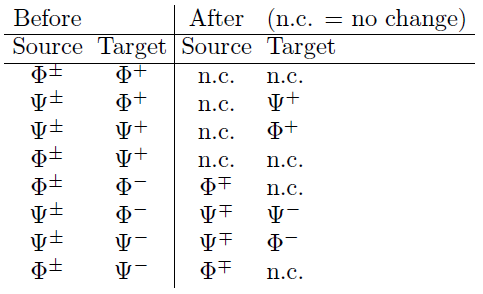
\includegraphics[width=100mm,keepaspectratio]{bennetoperations}
\caption[BXOR hatása Bell állapotokra]{BXOR hatása Bell-állapotokra.}
\end{figure}
-Az előző unitér transzformációkon kívül alkalmazunk még egy mérést is, melyben Alíz és Bob a z tengely mentén mér (elektronok spinjeit), amivel megbízhatóan meg tudjuk különböztetni a $\Phi$ és $\Psi$ állapotokat, viszont a ``-'' és ``+'' -t nem. Természetesen a mérés után a mért pár már nincs összefonódott állapotban.
Ezen műveletek birtokában tekintsük az alábbi protokollt, melynek bemenetei valamilyen F tisztaságú Werner állapotok:
\begin{enumerate}
\item Egy unilateláris $\sigma_y$ forgatást hajtunk végre mind a két páron, aminek hatására a többnyire $\Psi^-$ Werner állapotból a többnyire $\Phi^+$ Werner állapotba kerülnek.
\item Végrehajtunk egy  BXOR-t a két nem tiszta $\Phi^+$ állapoton és utána a célpárt megmérjük a z tengely mentén. Ha a mérési eredmények párhuzamosak, ami a $\Phi^+$ állapotnak megfelelő, akkor a meg nem mért forráspárt  megtartjuk, ellenkező esetben nem.
\item Végül, ha a forráspárt megtartottuk, egy többnyire $\Psi^-$ állapotba visszaalakítjuk egy unilaterális $\sigma_y$ forgatással, majd forgásszimmetrikussá tesszük egy véletlen bilaterális forgatással.
\end{enumerate}
Ezen egyszerű protokoll ismétlésével lépésenként legalább ¼-ed valószínűséggel növekvő F tisztaságot lehet elérni, amennyiben a felhasznált $M$ párokra igaz, hogy
$F_m > 1/2$  . Továbbá a lépésenként így elért $F'>F$ kielégíti a következő egyenletet:\\
\begin{center}
$F' = \frac{F^2 + \frac{1}{9}(1-F)^2}{F^2 + \frac{2}{3}F(1-F) + \frac{5}{9}(1-F)^2} $
\end{center}
A módszer ismételt elvégzésével a tiszta állapotot tetszőlegesen megközelítő állapot állítható elő, viszont a hatékonyság (nem tiszta bemenet/tiszta kimenet)  a teljesen tiszta kimenet közelítésével a 0-hoz tart. Ennek a javítására szerencsére vannak módszerek, egy ilyen lehetőség például, ha nem egy forrást párt BXOR-olunk egy célpárral, hanem többet. Ennek az ötletnek egy továbbfejlesztése, amikor tiszta $\Phi^+$  állapotokat használunk a BXOR céljaként a több nem tiszta forráspárhoz. Ezután megmérjük a célt. A fenti tábla alapján minden $\Psi^+$ vagy $\Psi^-$ forráspár váltja a célt $\Phi^+$ és $\Psi^+$ között, a forrásra való hatás nélkül. Ennek alapján a BXOR-t egyfajta paritás tesztként használva meg tudjuk állapítani, hogy a mért halmazban páratlan vagy páros számú $\Psi$ állapot van. Ezután további BXOR-ok elvégzésével a részhalmazokon, kiválasztható az összes $\Psi$ állapot és $\Phi$ állapotra javítható, majd hasonló módszerrel meg lehet találni a $\Phi^-$ állapotokat is és javítani a kívánt $\Phi^+$-ra.\\
Természetesen léteznek más tisztítóprotokollok is más tulajdonságokkal, viszont a továbbiakhoz nem szükséges ezen terület mélyebb ismerete.% lehet tisztítóprot forrásokat ide.
\\
Az ismétlő következő eleme maga a Bell-mérés aminek következtében maga az ``összefonódás megosztás'' nevű jelenség a párokon ténylegesen végbe megy. Megemlítendő, hogy amennyiben nem teljesen tiszta állapotokat mérünk ennek hatására a létrejövő új pár tisztasága is romlani fog, valamint magának a mérésnek is lehet egy hibaszázaléka \cite{lutkenhaus1999bell}, amiket a későbbi lépésekben ugyanúgy javítani kell.\\
Fontos elemek még az állomásokon található kvantumos állapotok tárolására képes memóriaegységek. Mivel a végső cél az ismétlő két végén található memóriában tárolt qubit közötti összefonódás létrehozása, természetes feltétel az állapothű tároláson túl, hogy ezek a memóriák képesek legyenek megtartani a qubit állapotát a protokoll végigfutási ideje alatt. Az alkalmazható hibajavítási stratégiáknak ez is egyfajta gátat szab mint az összes rendszerben tölthető idő felső határa. \\
\begin{figure}[h]
\centering
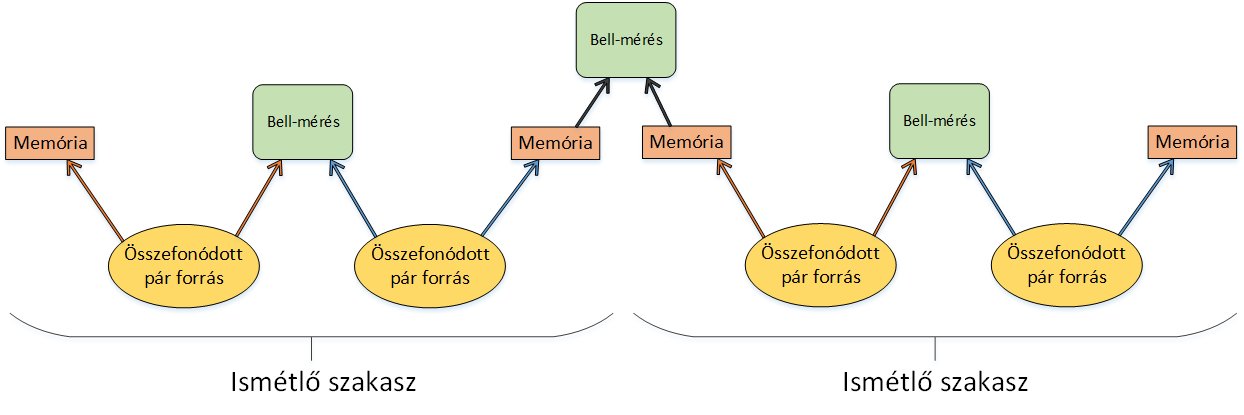
\includegraphics[width=\textwidth,keepaspectratio]{repeater}
\caption[Általános ismétlő]{Általános ismétlő rajza\\ A tisztító protokoll a képen nincs feltüntetve, tipikusan a Bell-mérések előtt alkalmazzák, habár ettől eltérő stratégiák is létezhetnek.}
\end{figure}

\subsection{Néhány megvalósítás}

A továbbiakban vizsgáljunk néhány mostani megvalósítást, ahol már láthatóak a technológia alkalmazásából származó előnyök valamint kihívások is.\\
Egy 2016-os német tanulmányban\cite{uphoff2016integrated} atom-foton összefonódott párokat használnak, melyeket optikai mikroüregekben található magányos atomok segítségével hoznak létre. Az összefonódás közvetlen az atomi kvantummemória és a foton között jön létre. További előny még, hogy ennek létrejöttét egy másik ún. “bejelentő” foton is jelzi és az összefonódást szállító foton olyan előnyös tulajdonságokkal rendelkezik (spektrum stb), hogy az egész elrendezés a szokványos telekommunikációs hullámhossztartományban használható. A további lépések az általános modellt követik, maga az összefonódás megosztás, fotonok közötti Bell-mérésekkel, és atom-atom kapuk alkalmazásával történik.
\begin{figure}[H]
\centering
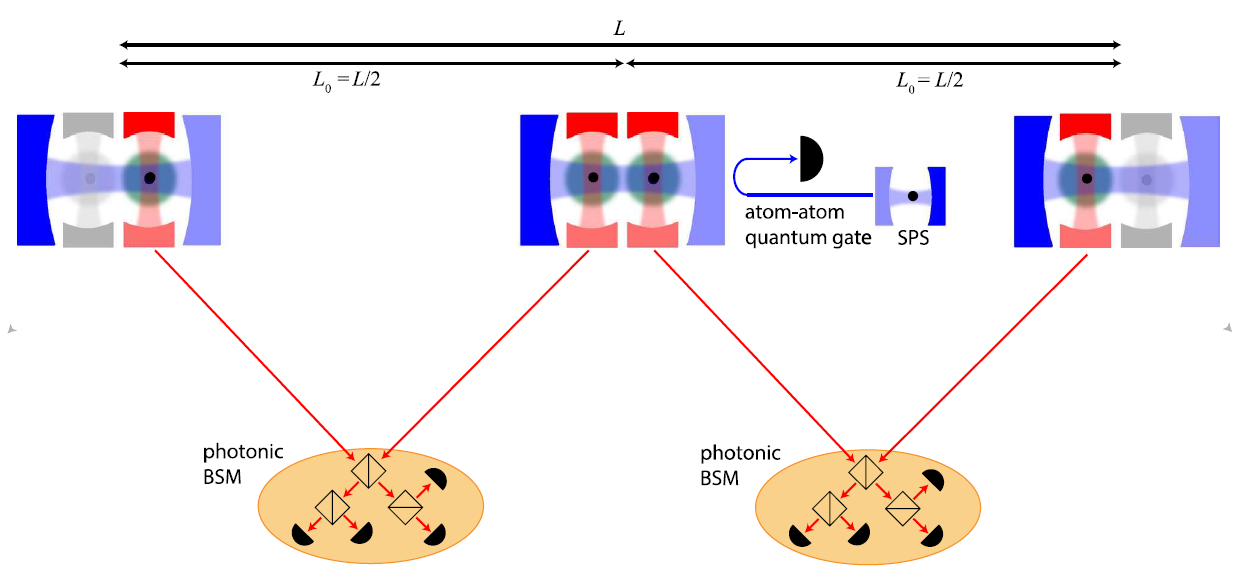
\includegraphics[width=\textwidth,keepaspectratio]{nemetkis}
\caption[Atom-foton ismétlő elvi rajza]{A 2016-os német tanulmány elvi rajza.\\
Egy ismétlő csomópont a “bejelentő” üregből(kék) és telekommunikációs hullámhosszú összefonó üregekből áll. Az atomokat (fekete pont) lézersugarakkal irányítjuk. Az L/2 távolságra lévő csomópontokat először összefonódott állapotba juttatjuk a fotonokon elvégzett (L/4 távolságnál) Bell-mérések segítségével. A csomópont párok között összefonódás megosztást a központi csomópontban elvégzett (atom-atom) művelettel valósítjuk meg.   
}
\end{figure}
A tanulmány szépen szemlélteti még a távolságból és a hibajavításból adódó problémák hatását.
\begin{figure}[H]
\centering
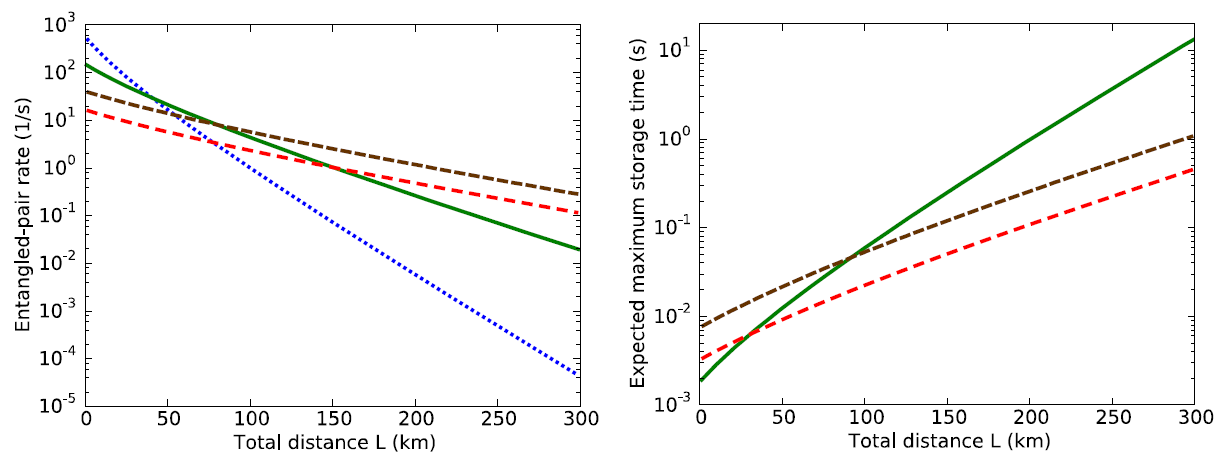
\includegraphics[width=\textwidth,keepaspectratio]{nemetgraph}
\caption[Ismétlő teljesítmény]{A várható átviteli sebesség és tárolási idő alakulása az áthidalni kívánt távolság függvényében.\\
Kék pontozott vonal-> ismétlő nélküli eset; zöld folytonos vonal->2 szakasz esetén\\
piros szaggatott vonal-> 4 szakasz esetén, hibánál teljes újrakezdéssel\\
barna szaggatott vonal-> 4 szakasz hibánál a már összefonódott állapotok megtartásával\\
}
\end{figure}

Látszik, hogy kis távolságoknál a közvetlen összeköttetés a legjobb egyszerűsége miatt, viszont 100km fölött már számottevően jobbak az ismétlős megoldások. A tárolási idő szempontjából látszik, hogy nagy távolságoknál a több részre felosztott rendszerek teljesítenek jobban. (Továbbá az is, hogy a hiba teljes újrakezdéssel való javítása is meglehetősen csökkenti a szükséges tárolási időt.)\\
Egy másik 2016-os tanulmány \cite{krovi2016practical} az ún. ``parametric down conversion'' jelenséget és két foton interferenciát hasznosító  összefonódott pár forrásokat használó jelen/közeli jövőbeli ismétlők lehetséges korlátjait vizsgálta, különös tekintettel az egyszerű megvalósíthatóságra a mai technológiákkal. Az ő szimulációjukból is látszik az ismétlők előnye nagyobb távolságok esetén:\\
\begin{figure}[H]
\centering
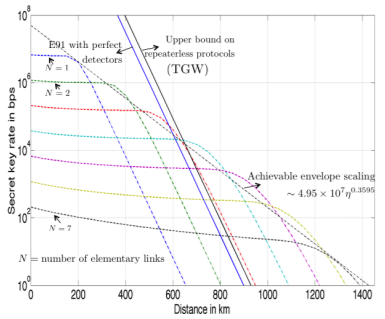
\includegraphics[width=100mm,keepaspectratio]{othergraph}
\caption[Ismétlő teljesítményhatár]{A különböző számú kapcsolatokból álló ismétlőrendszerek átvitele és összehasonlításuk más ismétlő nélküli protokollok határaival (TGW vonal ezek felső határa).
}
\end{figure}
Különböző ismétlő protokollok akár ionokkal való megvalósítási lehetőségét is vizsgálták \cite{pfister2016quantum} ugyancsak 2016-ban. Az általuk használt kísérleti összeállításban $^{40}Ca^+$ ionok segítségével már F>0.95 esetén 100 állapot/s sebességet is elértek bizonyos protokollok esetén, azonban megfelelő változtatásokkal a több mint 750 állapot/s sebességet is elérhetőnek találták, az ionos megvalósítások esetében.\\

Egy negyedik, kínai tanulmány \cite{li2016heralded} pedig a kvantum pontok és optikai üregek használatával való megvalósítással foglalkozik. Ennek egyik érdekessége, hogy itt úgynevezett time-bin összefonódást hoznak létre, aminek folyamán a fotonoknak az időbeli szabadságfokát használják fel információtárolásra. 
A tanulmányban továbbá megmutatják, egy lehetséges $N$ többfelhasználós kvantum ismétlő rendszer felépítését is.

\section{Összefoglaló}

Már az említett megvalósításokból is látszik, hogy a kísérleti kvantuminformációs megvalósítások hatékonysága, erőforrásigénye és megbízhatósága egyre inkább közelíti a gyakorlatban való eredményes használhatósághoz szükséges feltételek teljesítését az információszétosztás területén is. Tekintve a terület gyors fejlődését, különösen, hogy a kvantum titkosítás és kulcsszétosztás már a jelenben is gyakorlati jelentőséggel bír, a kvantum ismétlők ipari megvalósítása nagy valószínűséggel már a közeljövőben is egy megoldandó mérnöki feladatot fog jelenteni. A fentebb szemléltetett tervezésnél megfontolandó nehézségek fényében döntöttem egy szimuláció elkészítése mellett, ahol a továbbiakban ezek hatását szemléltetem illetve vizsgálom.
